\documentclass{standalone}
\usepackage{tikz}
\usetikzlibrary{patterns, positioning}


\begin{document}
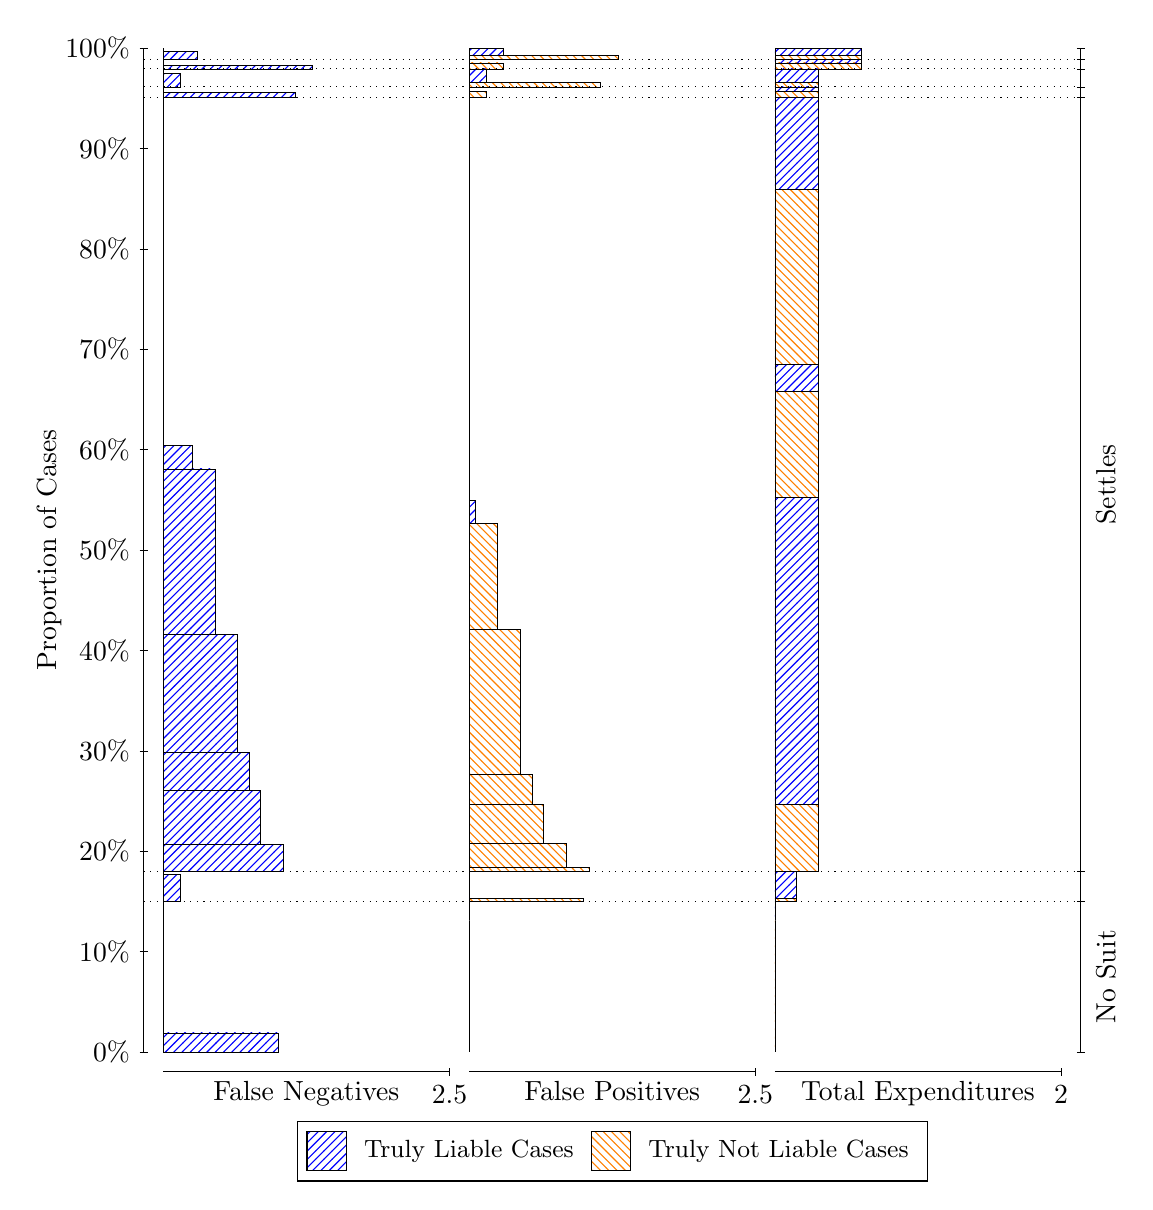
\begin{tikzpicture}
\draw[black, very thin] (1.5,1.75) -- (1.5,14.5);
\node[rotate=90, text=black, anchor=center] at (0.3, 8.125) {Proportion of Cases};
\draw[black, very thin] (1.45,1.75) -- (1.55,1.75);
\node[text=black, anchor=east] at (1.45, 1.75) {0\%};
\draw[black, very thin] (1.45,3.025) -- (1.55,3.025);
\node[text=black, anchor=east] at (1.45, 3.025) {10\%};
\draw[black, very thin] (1.45,4.3) -- (1.55,4.3);
\node[text=black, anchor=east] at (1.45, 4.3) {20\%};
\draw[black, very thin] (1.45,5.575) -- (1.55,5.575);
\node[text=black, anchor=east] at (1.45, 5.575) {30\%};
\draw[black, very thin] (1.45,6.85) -- (1.55,6.85);
\node[text=black, anchor=east] at (1.45, 6.85) {40\%};
\draw[black, very thin] (1.45,8.125) -- (1.55,8.125);
\node[text=black, anchor=east] at (1.45, 8.125) {50\%};
\draw[black, very thin] (1.45,9.4) -- (1.55,9.4);
\node[text=black, anchor=east] at (1.45, 9.4) {60\%};
\draw[black, very thin] (1.45,10.675) -- (1.55,10.675);
\node[text=black, anchor=east] at (1.45, 10.675) {70\%};
\draw[black, very thin] (1.45,11.95) -- (1.55,11.95);
\node[text=black, anchor=east] at (1.45, 11.95) {80\%};
\draw[black, very thin] (1.45,13.225) -- (1.55,13.225);
\node[text=black, anchor=east] at (1.45, 13.225) {90\%};
\draw[black, very thin] (1.45,14.5) -- (1.55,14.5);
\node[text=black, anchor=east] at (1.45, 14.5) {100\%};

\draw[black, very thin] (13.4,1.75) -- (13.4,14.5);
\draw[black, very thin] (13.35,1.75) -- (13.45,1.75);
\node[anchor=west] at (13.35, 1.75) {};
\draw[black, very thin] (13.35,3.6618) -- (13.45,3.6618);
\node[anchor=west] at (13.35, 3.6618) {};
\draw[black, very thin] (13.35,4.0429) -- (13.45,4.0429);
\node[anchor=west] at (13.35, 4.0429) {};
\draw[black, very thin] (13.35,13.87) -- (13.45,13.87);
\node[anchor=west] at (13.35, 13.87) {};
\draw[black, very thin] (13.35,14.007) -- (13.45,14.007);
\node[anchor=west] at (13.35, 14.007) {};
\draw[black, very thin] (13.35,14.235) -- (13.45,14.235);
\node[anchor=west] at (13.35, 14.235) {};
\draw[black, very thin] (13.35,14.356) -- (13.45,14.356);
\node[anchor=west] at (13.35, 14.356) {};
\draw[black, very thin] (13.35,14.5) -- (13.45,14.5);
\node[anchor=west] at (13.35, 14.5) {};

\draw[black, very thin, pattern color=blue, pattern=north east lines] (1.75,1.75) rectangle (3.2033,1.9926);
\draw[black, very thin, pattern color=orange, pattern=north west lines] (1.75,1.9926) rectangle (1.75,3.6618);
\draw[black, very thin, pattern color=blue, pattern=north east lines] (1.75,3.6618) rectangle (1.968,4.0063);
\draw[black, very thin, pattern color=orange, pattern=north west lines] (1.75,4.0063) rectangle (1.75,4.0429);
\draw[black, very thin, pattern color=blue, pattern=north east lines] (1.75,4.0429) rectangle (3.276,4.3816);
\draw[black, very thin, pattern color=blue, pattern=north east lines] (1.75,4.3816) rectangle (2.9853,5.0758);
\draw[black, very thin, pattern color=blue, pattern=north east lines] (1.75,5.0758) rectangle (2.84,5.5502);
\draw[black, very thin, pattern color=blue, pattern=north east lines] (1.75,5.5502) rectangle (2.6947,7.0487);
\draw[black, very thin, pattern color=blue, pattern=north east lines] (1.75,7.0487) rectangle (2.404,9.1542);
\draw[black, very thin, pattern color=blue, pattern=north east lines] (1.75,9.1542) rectangle (2.1133,9.4507);
\draw[black, very thin, pattern color=orange, pattern=north west lines] (1.75,9.4507) rectangle (1.75,13.87);
\draw[black, very thin, pattern color=blue, pattern=north east lines] (1.75,13.87) rectangle (3.4213,13.933);
\draw[black, very thin, pattern color=orange, pattern=north west lines] (1.75,13.933) rectangle (1.75,14.007);
\draw[black, very thin, pattern color=blue, pattern=north east lines] (1.75,14.007) rectangle (1.968,14.181);
\draw[black, very thin, pattern color=orange, pattern=north west lines] (1.75,14.181) rectangle (1.75,14.235);
\draw[black, very thin, pattern color=blue, pattern=north east lines] (1.75,14.235) rectangle (3.6393,14.281);
\draw[black, very thin, pattern color=orange, pattern=north west lines] (1.75,14.281) rectangle (1.75,14.356);
\draw[black, very thin, pattern color=blue, pattern=north east lines] (1.75,14.356) rectangle (2.186,14.454);
\draw[black, very thin, pattern color=orange, pattern=north west lines] (1.75,14.454) rectangle (1.75,14.5);
\draw[black, very thin, pattern color=orange, pattern=north west lines] (5.6333,1.75) rectangle (5.6333,3.4192);
\draw[black, very thin, pattern color=blue, pattern=north east lines] (5.6333,3.4192) rectangle (5.6333,3.6618);
\draw[black, very thin, pattern color=orange, pattern=north west lines] (5.6333,3.6618) rectangle (7.0867,3.6984);
\draw[black, very thin, pattern color=blue, pattern=north east lines] (5.6333,3.6984) rectangle (5.6333,4.0429);
\draw[black, very thin, pattern color=orange, pattern=north west lines] (5.6333,4.0429) rectangle (7.1593,4.0985);
\draw[black, very thin, pattern color=orange, pattern=north west lines] (5.6333,4.0985) rectangle (6.8687,4.3959);
\draw[black, very thin, pattern color=orange, pattern=north west lines] (5.6333,4.3959) rectangle (6.578,4.8963);
\draw[black, very thin, pattern color=orange, pattern=north west lines] (5.6333,4.8963) rectangle (6.4327,5.2796);
\draw[black, very thin, pattern color=orange, pattern=north west lines] (5.6333,5.2796) rectangle (6.2873,7.1198);
\draw[black, very thin, pattern color=orange, pattern=north west lines] (5.6333,7.1198) rectangle (5.9967,8.4626);
\draw[black, very thin, pattern color=blue, pattern=north east lines] (5.6333,8.4626) rectangle (5.706,8.759);
\draw[black, very thin, pattern color=blue, pattern=north east lines] (5.6333,8.759) rectangle (5.6333,13.87);
\draw[black, very thin, pattern color=orange, pattern=north west lines] (5.6333,13.87) rectangle (5.8513,13.945);
\draw[black, very thin, pattern color=blue, pattern=north east lines] (5.6333,13.945) rectangle (5.6333,14.007);
\draw[black, very thin, pattern color=orange, pattern=north west lines] (5.6333,14.007) rectangle (7.3047,14.061);
\draw[black, very thin, pattern color=blue, pattern=north east lines] (5.6333,14.061) rectangle (5.8513,14.235);
\draw[black, very thin, pattern color=orange, pattern=north west lines] (5.6333,14.235) rectangle (6.0693,14.31);
\draw[black, very thin, pattern color=blue, pattern=north east lines] (5.6333,14.31) rectangle (5.6333,14.356);
\draw[black, very thin, pattern color=orange, pattern=north west lines] (5.6333,14.356) rectangle (7.5227,14.402);
\draw[black, very thin, pattern color=blue, pattern=north east lines] (5.6333,14.402) rectangle (6.0693,14.5);
\draw[black, very thin, pattern color=orange, pattern=north west lines] (9.5167,1.75) rectangle (9.5167,3.4192);
\draw[black, very thin, pattern color=blue, pattern=north east lines] (9.5167,3.4192) rectangle (9.5167,3.6618);
\draw[black, very thin, pattern color=orange, pattern=north west lines] (9.5167,3.6618) rectangle (9.7892,3.6984);
\draw[black, very thin, pattern color=blue, pattern=north east lines] (9.5167,3.6984) rectangle (9.7892,4.0429);
\draw[black, very thin, pattern color=orange, pattern=north west lines] (9.5167,4.0429) rectangle (10.062,4.8963);
\draw[black, very thin, pattern color=blue, pattern=north east lines] (9.5167,4.8963) rectangle (10.062,8.7968);
\draw[black, very thin, pattern color=orange, pattern=north west lines] (9.5167,8.7968) rectangle (10.062,10.14);
\draw[black, very thin, pattern color=blue, pattern=north east lines] (9.5167,10.14) rectangle (10.062,10.478);
\draw[black, very thin, pattern color=orange, pattern=north west lines] (9.5167,10.478) rectangle (10.062,12.702);
\draw[black, very thin, pattern color=blue, pattern=north east lines] (9.5167,12.702) rectangle (10.062,13.87);
\draw[black, very thin, pattern color=orange, pattern=north west lines] (9.5167,13.87) rectangle (10.062,13.945);
\draw[black, very thin, pattern color=blue, pattern=north east lines] (9.5167,13.945) rectangle (10.062,14.007);
\draw[black, very thin, pattern color=orange, pattern=north west lines] (9.5167,14.007) rectangle (10.062,14.061);
\draw[black, very thin, pattern color=blue, pattern=north east lines] (9.5167,14.061) rectangle (10.062,14.235);
\draw[black, very thin, pattern color=orange, pattern=north west lines] (9.5167,14.235) rectangle (10.607,14.31);
\draw[black, very thin, pattern color=blue, pattern=north east lines] (9.5167,14.31) rectangle (10.607,14.356);
\draw[black, very thin, pattern color=orange, pattern=north west lines] (9.5167,14.356) rectangle (10.607,14.402);
\draw[black, very thin, pattern color=blue, pattern=north east lines] (9.5167,14.402) rectangle (10.607,14.5);
\draw[black, dotted] (1.5,3.6618) -- (13.4,3.6618);
\draw[black, dotted] (1.5,4.0429) -- (13.4,4.0429);
\draw[black, dotted] (1.5,13.87) -- (13.4,13.87);
\draw[black, dotted] (1.5,14.007) -- (13.4,14.007);
\draw[black, dotted] (1.5,14.235) -- (13.4,14.235);
\draw[black, dotted] (1.5,14.356) -- (13.4,14.356);
\draw[black, very thin] (1.75,1.5) -- (5.3833,1.5);
\node[text=black, anchor=north] at (3.5667, 1.5) {False Negatives};
\draw[black, very thin] (5.3833,1.45) -- (5.3833,1.55);
\node[text=black, anchor=north] at (5.3833, 1.45) {2.5};

\draw[black, very thin] (5.6333,1.5) -- (9.2667,1.5);
\node[text=black, anchor=north] at (7.45, 1.5) {False Positives};
\draw[black, very thin] (9.2667,1.45) -- (9.2667,1.55);
\node[text=black, anchor=north] at (9.2667, 1.45) {2.5};

\draw[black, very thin] (9.5167,1.5) -- (13.15,1.5);
\node[text=black, anchor=north] at (11.333, 1.5) {Total Expenditures};
\draw[black, very thin] (13.15,1.45) -- (13.15,1.55);
\node[text=black, anchor=north] at (13.15, 1.45) {2};

\node[text=black, centered, rotate=90] at (13.72, 2.7059) {No Suit};

\node[text=black, centered, rotate=90] at (13.72, 8.9566) {Settles};





\draw (7.449999999999999,1.5) node[draw=none] (baseCoordinate) {};
\begin{scope}[align=center]
        \matrix[scale=0.5, draw=black, below=0.5cm of baseCoordinate, nodes={draw}, column sep=0.1cm]{
            \node[rectangle, draw, minimum width=0.5cm, minimum height=0.5cm, pattern color=blue, pattern=north east lines] {}; &
            \node[draw=none, font=\small, text=black] (B) {Truly Liable Cases}; &
            \node[rectangle, draw, minimum width=0.5cm, minimum height=0.5cm, pattern color=orange, pattern=north west lines] {}; &
            \node[draw=none, font=\small, text=black] (B) {Truly Not Liable Cases}; \\
            };
\end{scope}

\end{tikzpicture}
\end{document}